\section*{Introduction}
\label{707961}

Medical decision-making is a complex cognitive process in which clinicians interpret clinical information and arrive at diagnostic or treatment decisions. Disagreement among professionals is common, even when they evaluate the same data. Understanding the sources of this disagreement is essential for improving diagnostic reliability and accuracy, designing effective training interventions, and determining appropriate sample sizes in clinical research.

Inter- and intra-rater disagreement reflects both (i) variation in the underlying signal (i.e., genuine differences in case difficulty) and (ii) noise (i.e., unwanted variability in judgment). Traditional reliability metrics such as Cohen’s kappa or intraclass correlation coefficients quantify \textit{how much} experts disagree, but they provide little insight into \textit{why}. For example, a kappa of 0.65 indicates “moderate agreement,” yet it does not indicate whether disagreement arises from differing thresholds, idiosyncratic feature weighting, instability within raters over time, or random inconsistency. Without identifying the sources of disagreement, it is difficult to design targeted interventions to improve reliability and accuracy.

Recent work in decision science \cite{Kahneman2021} distinguishes multiple types of noise: \textit{level noise} (systematic differences in how lenient or stringent raters are), \textit{pattern noise} (idiosyncratic differences in how raters weigh features of individual cases), and \textit{occasion noise} (inconsistency within the same rater across repeated assessments of identical information). Each noise type suggests different remedies: level noise motivates threshold calibration, pattern noise motivates case-based training, and occasion noise motivates environmental controls or decision support tools.

Consider two clinicians who disagree on whether a patient has epilepsy. Is the disagreement because one clinician is generally more conservative (level noise), because they weight clinical evidence differently (pattern noise), or because one clinician is inconsistent across repeated assessments (occasion noise)? Standard agreement metrics cannot distinguish among these possibilities. This paper provides a “diagnostic tool for diagnostic systems”: a framework that decomposes disagreement into interpretable, actionable components.

We present a unified statistical framework for quantifying sources of variation in binary medical decisions such as “Does this patient have epilepsy?” or “Is this waveform epileptiform?” We show that the latent trait model (LTM) and the Kahneman--Sibony--Sunstein (KSS) noise decomposition framework can be understood as special cases of a single generalized linear mixed model (GLMM). We demonstrate the framework using data from an experiment in which 20 expert neurologists evaluated 50 cases for epilepsy diagnosis \cite{nascimentonoise}. We provide practical guidance for applied researchers on model implementation, interpretation, and study design. A key result is that discrimination ability (as measured by area under the ROC curve) depends only on pattern and occasion noise, whereas threshold choice (the operating point on the ROC curve) is governed by level noise.

\subsection*{Overview: Inputs, Outputs, and Use Cases}

To orient applied readers, we summarize what the method requires, what it produces, and when it is useful.

\begin{table}[h!]
\centering
\small
\begin{tabular}{p{0.25\textwidth}p{0.65\textwidth}}
\toprule
\textbf{Component} & \textbf{Description} \\
\midrule
\multicolumn{2}{l}{\textbf{INPUTS}} \\
Binary ratings & Response array $Y_{ijt}$: ratings from $M$ raters on $N$ cases, optionally repeated over $T$ occasions \\
Sample sizes & Typical: $N \geq 30$ cases, $M \geq 10$ raters; $T \geq 2$ occasions if estimating occasion noise \\
Gold standard (optional) & Reference labels for evaluating accuracy (sensitivity/specificity); not required for noise decomposition \\
\midrule
\multicolumn{2}{l}{\textbf{PRIMARY OUTPUTS}} \\
Variance components & Standard deviations $\sigma_c, \sigma_\ell, \sigma_p, \sigma_o$ quantifying signal, level noise, pattern noise, and occasion noise \\
Percent contributions & Proportion of total variation explained by each component \\
Uncertainty & Credible intervals (Bayesian) or confidence intervals (frequentist) for all estimates \\
\midrule
\multicolumn{2}{l}{\textbf{SECONDARY OUTPUTS}} \\
Rater-level summaries & Individual estimates of level noise, pattern noise, occasion noise for each rater \\
Case-level summaries & Predicted consensus probability for each case \\
Model validation & Posterior predictive checks, goodness-of-fit diagnostics \\
\midrule
\multicolumn{2}{l}{\textbf{USE CASES}} \\
1. Quantify disagreement & Separate signal from noise; identify specific noise sources \\
2. Compare groups & Test whether/how experts vs.\ non-experts differ in level, pattern, or occasion noise \\
3. Design studies & Determine required sample sizes (cases, raters, repeats) \\
4. Evaluate training & Measure changes in noise components before/after training interventions \\
5. Quality assurance & Identify raters with excessive noise or miscalibration \\
\bottomrule
\end{tabular}
\caption{Summary of inputs, outputs, and use cases for the noise decomposition framework.}
\label{tab:overview}
\end{table}

\subsection*{Why Decomposition Matters: An Illustrative Example}

Figure~\ref{fig:killer} illustrates why decomposing noise into its components is clinically valuable. We simulated two raters evaluating the same cases on three occasions, assuming equal numbers of positive and negative cases but varying case difficulty. The variation in the underlying signal (degree of evidence pointing to the correct diagnosis) is represented by $\sigma_c$. Both raters see identical information, but their judgments are affected by different amounts and types of noise:

\beg


% \section*{Introduction}

% {\label{707961}}

% Medical decision-making refers to the complex cognitive process whereby medical professionals interpret clinical information and arrive at diagnostic or treatment decisions. Disagreement among professionals in making medical decisions is not uncommon. Understanding the sources of this disagreement is critical for improving diagnostic reliability and accuracy, designing clinical training programs, and determining appropriate sample sizes in clinical research.

% Inter- and intra-rater disagreement arises both from noise (i.e., unwanted variability) and the underlying signal (i.e., variability derived from genuine differences in case difficulty). While traditional reliability metrics such as Cohen's kappa or intraclass correlation coefficients tell us \textit{how much} experts disagree, they fail to inform us why. For instance, a kappa of 0.65 indicates ``moderate agreement'', but provides no insight into whether disagreement stems from varying case difficulty, differing personal thresholds, idiosyncratic interpretations of evidence, or random inconsistency. Without understanding the precise sources of disagreement, we cannot design targeted interventions to improve accuracy and reliability.

% Recent work in decision science \cite{Kahneman2021} has identified distinct types of noise: \textit{level noise} (systematic differences in how lenient or stringent raters are), \textit{pattern noise} (idiosyncratic differences in how raters weigh features of individual cases), and \textit{occasion noise} (inconsistency within the same rater across repeated assessments of the same data). Crucially, each noise type suggests different remedies: level noise calls for threshold calibration, pattern noise for case-based training, and occasion noise for environmental control and decision support tools.

% Consider two clinicians who disagree on whether a patient has epilepsy. Is the disagreement because one expert is generally more conservative in diagnosing epilepsy (level noise), or because they give different weights to different aspects of the case (pattern noise), or because one expert is having an "off day" (occasion noise)? Traditional reliability metrics cannot answer this question. This paper provides a "diagnostic tool for diagnostic systems"--- a framework to decompose disagreement into quantifiable, actionable components.

% We present a unified statistical framework for quantifying the sources of variation in binary medical decisions such as, "Does this patient have epilepsy?" or "Is this waveform epileptiform?". We show how the latent trait model (LTM) and the Kahneman-Sibony-Sunstein (KSS) noise decomposition framework can be understood as special cases of a single generalized linear mixed model (GLMM). We demonstrate the framework using data from an experiment where 20 expert neurologists evaluated 50 cases for epilepsy diagnosis \cite{nascimentonoise}. We provide practical guidance for applied researchers on how to implement these models, interpret the results, and design studies to estimate noise components reliably. We show that discrimination ability (reflected in the area under the ROC curve) depends only on pattern noise and occasion noise, while threshold choice (the operating point on the ROC curve) is determined by level noise.

% \subsection*{Overview: Inputs, Outputs, and Use Cases}

% To orient applied readers, we first summarize what this method requires, what it produces, and when it is useful.

% \begin{table}[h!]
% \centering
% \small
% \begin{tabular}{p{0.25\textwidth}p{0.65\textwidth}}
% \toprule
% \textbf{Component} & \textbf{Description} \\
% \midrule
% \multicolumn{2}{l}{\textbf{INPUTS}} \\
% Binary ratings & Response array $Y_{ijt}$: ratings from $M$ raters on $N$ cases, optionally repeated over $T$ occasions \\
% Sample sizes & Typical: $N \geq 30$ cases, $M \geq 10$ raters; $T \geq 2$ occasions if estimating occasion noise \\
% Gold standard (optional) & Reference labels for evaluating accuracy (sensitivity/specificity); not required for noise decomposition \\
% \midrule
% \multicolumn{2}{l}{\textbf{PRIMARY OUTPUTS}} \\
% Variance components & Standard deviations $\sigma_c, \sigma_\ell, \sigma_p, \sigma_o$ quantifying signal, level noise, pattern noise, and occasion noise \\
% Percent contributions & Proportion of total variation explained by each component \\
% Uncertainty & Credible intervals (Bayesian) or confidence intervals (frequentist) for all estimates \\
% \midrule
% \multicolumn{2}{l}{\textbf{SECONDARY OUTPUTS}} \\
% Rater-level summaries & Individual estimates of level noise, pattern noise, occasion noise for each rater \\
% Case-level summaries & Predicted consensus probability for each case \\
% Model validation & Posterior predictive checks, goodness-of-fit diagnostics \\
% \midrule
% \multicolumn{2}{l}{\textbf{USE CASES}} \\
% 1. Quantify disagreement & Separate signal from noise; identify specific noise sources \\
% 2. Compare groups & Test whether/how experts vs. non-experts differ in level, pattern, or occasion noise \\
% 3. Design studies & Determine required sample sizes (cases, raters, repeats) \\
% 4. Evaluate training & Measure changes in noise components before/after training interventions \\
% 5. Quality assurance & Identify raters with excessive noise or miscalibration \\
% \bottomrule
% \end{tabular}
% \caption{Summary of inputs, outputs, and use cases for the noise decomposition framework.}
% \label{tab:overview}
% \end{table}

% \subsection*{Why Decomposition Matters: An Illustrative Example}

% Figure~\ref{fig:killer} illustrates why decomposing noise into its components is clinically valuable. We simulated two raters evaluating the same cases, on three occasions. We assume an equal number of positive and negative cases, but that case difficulty varies, and the variation in the underlying signal (degree of evidence pointing to the correct diagnosis) is represented by $\sigma_c$. The two raters see the same information, but their judgments are clouded by different anmounts and types of noise:

% \begin{itemize}
%     \item \textbf{Rater A ("Stringent but consistent"):} Low pattern noise ($\sigma_p = 0.66$) and occasion noise ($\sigma_o = 0.44$) result in \textit{superior} discrimination (AUC = 0.78)---this rater has substantially better ability to distinguish positive from negative cases compared to rater B. However,  rater A has a systematically conservative threshold ($\ell = 2.0$), yielding low sensitivity (29\%) and high specificity (95\%, FPR = 5\%), with overall accuracy of 62\%. If this rater adjusted their threshold to the optimal value, they could achieve 71\% accuracy; they are wasting 9 percentage points of potential accuracy due to systematic underdiagnosis. This demonstrates that threshold optimization alone can improve accuracy without changing discrimination ability.

%     \item \textbf{Rater B ("Lenient but inconsistent"):} Lower skill, reflected in higher pattern noise ($\sigma_p = 0.97$) and occasion noise ($\sigma_o = 0.65$) result in \textit{inferior} discrimination (AUC = 0.70)---rater B's ability to distinguish positive from negative cases is worse than Rater A's. However, this rater has a well-calibrated threshold ($\ell = 0.2$), producing balanced sensitivity (64\%) and specificity (64\%, false positive rate = 36\%), yielding accuracy of 64\%, better than Rater A. Rater B is already operating at their optimal threshold and cannot improve accuracy without improving in skill, which means reducing discrimination noise (by reducing pattern and occasion noise). This shows that inferior discrimination with an optimal threshold can yield higher accuracy than superior discrimination with a miscalibrated threshold.
% \end{itemize}

% The heatmaps of responses (cases × occasions) in Figure 1 reveal the distinct noise patterns. Rater A shows systematic bias (a tendancy to undercall the positive class), while Rater B shows scattered disagreements. The ROC curves demonstrate that Rater A has the better ROC curve (higher AUC due to low pattern noise and occasion noise) but operates at a suboptimal point (white circle) due to conservative bias. Rater B has the worse ROC curve (lower AUC due to high pattern noise and occasion noise) but operates at a more well-calibrated point (black circle) due to unbiased threshold. Operating points show each rater's sensitivity-specificity trade-off.

% The stacked bars show signal and discrimination noise (pattern + occasion) as percentages of total response variance for each rater. Both raters see the same signal (same cases), but the percentages differ because they are relative to each rater's total variance. Rater A has lower total variance due to low discrimination noise, making signal represent a larger proportion. Rater B has higher total variance due to high discrimination noise. The variance decomposition reveals discrimination ability: Rater A has better discrimination (lower proportion of total response variation attributable to pattern and occasion noise) but an overly conservative threshold, while Rater B has poor discrimination (higher proportion of response variation explained by pattern and occasion noise) but good threshold calibration.

% \textbf{Clinical implications:}
% \begin{itemize}
%     \item For Rater A: Threshold recalibration (e.g., anchoring vignettes, feedback on diagnostic under-calling tendencies) is \textit{high priority}. The superior discrimination ability (AUC = 0.78) is being wasted due to a systematically very conservative threshold. Correcting the bias would improve accuracy from 62\% to 71\% (recovering 9 percentage points) without any change in discrimination (pattern noise and occasion noise). This is a \textit{low-cost, high-impact} intervention---no additional training required, just threshold adjustment. The large "wasted" potential (9 points) makes this especially urgent.
%     \item For Rater B: Case-based training (to reduce pattern noise) and decision aids (to reduce occasion noise) would improve discrimination, but are higher-cost interventions. Rater B is already operating at their optimal threshold (64\% accuracy), so they cannot improve further without reducing discrimination noise (pattern noise and occasion noise). Improving discrimination from AUC 0.70 to 0.78 would increase accuracy from 64\% to 71\%; however, this requires intensive training, unlike Rater A's "simple" threshold fix.
%     \item Traditional metrics focusing only on agreement or consistency would suggest Rater A is superior (less variable, higher AUC), missing that Rater A's superior discrimination is being undermined by poor threshold calibration while Rater B's inferior discrimination is being maximally utilized by optimal threshold choice. 
%     \item The key insight: Superior discrimination does not guarantee higher accuracy if threshold choice is suboptimal; conversely, inferior discrimination can yield higher accuracy if threshold choice is optimal. Noise decomposition reveals \textit{where} to intervene and \textit{how much} potential is being "wasted"---not just that intervention is needed.
% \end{itemize}

% In the example above, we have been comparing two individual clinicians, attributing their tendency to under- or over-diagnose cases as a fixed threshold, $\ell$, and we have noted that this threshold can vary between clinicians. When clinicians are viewed as a group, this unwanted threshold variation represents yet another form of noise, called \textit{level noise}. Thus, we have identified four sources of variation in the way clinicians may reach diagnoses: signal, and three sources of noise---level noise, pattern noise, and occasion noise. We now turn to how these can be measured and quantified.

% \begin{figure}[h!]
% \begin{center}
% 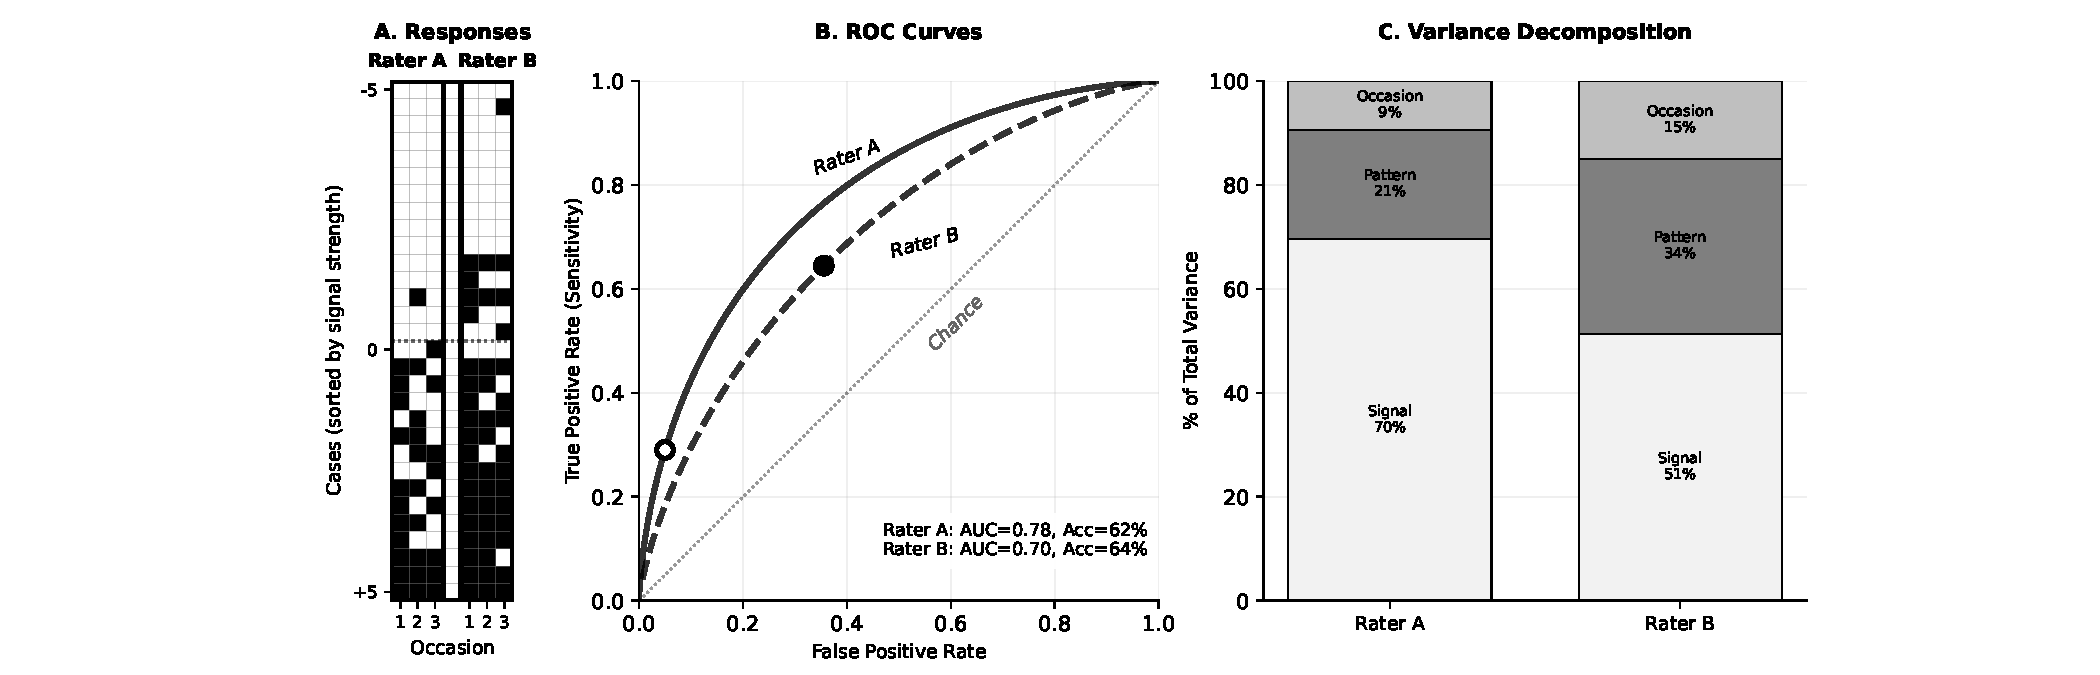
\includegraphics[width=1.0\textwidth]{killer_figure.pdf}
% \caption{\textbf{Superior discrimination with miscalibrated threshold yields lower accuracy than inferior discrimination with optimal threshold.} Two simulated raters evaluating the same cases (signal $\sigma_c = 1.2$ for both, prevalence = 50\%) with different noise profiles demonstrate why noise decomposition matters. \textbf{Panel A (Left):} Heatmaps of responses (30 cases × 3 occasions; white=negative, black=positive; cases sorted by difficulty; dotted line = true positive/negative boundary). Rater A (top) shows a clear tendency to under-call (systematic conservative bias), while Rater B (bottom) shows scattered disagreements reflecting inconsistency. \textbf{Panel B (Middle):} ROC curves from binormal model with discrimination ability (AUC) and actual accuracy (Acc) labeled on each curve. Rater A (solid line, AUC = 0.78) has substantially superior discrimination compared to Rater B (dashed line, AUC = 0.70). ROC curves reflect only pattern noise ($\sigma_p$) and occasion noise ($\sigma_o$)---\textit{not} threshold position ($\ell$). Operating points (circles) show where each rater operates on their respective curves. Rater A: low pattern noise ($\sigma_p = 0.66$) and occasion noise ($\sigma_o = 0.44$) yield superior discrimination (AUC = 0.78), but a systematically conservative threshold ($\ell = 2.0$) places them at a suboptimal operating point (white circle: sensitivity = 29\%, specificity = 95\%, FPR = 5\%), yielding only 62\% accuracy. With optimal threshold, this rater could achieve 71\% accuracy---\textit{wasting 9 percentage points due to threshold miscalibration}. Rater B: higher pattern noise ($\sigma_p = 0.97$) and occasion noise ($\sigma_o = 0.65$) yield inferior discrimination (AUC = 0.70), but a well-calibrated threshold ($\ell = 0.2$) produces a near-optimal operating point (black circle: sensitivity = 64\%, specificity = 64\%, FPR = 36\%), yielding 64\% accuracy---\textit{higher than Rater A despite worse discrimination}. Note that Rater A has higher AUC but lower accuracy than Rater B. \textbf{Panel C (Right):} Variance decomposition showing signal and discrimination noise as percentages of total response variance. Both raters see identical signal ($\sigma_c = 1.2$), but percentages differ because they are relative to each rater's total variance. Rater A has 54\% signal and 46\% discrimination noise (pattern + occasion); Rater B has 36\% signal and 64\% discrimination noise. The bars show only pattern and occasion noise (which together determine discrimination ability), not threshold position. The key insight: superior discrimination does not guarantee higher accuracy when threshold is miscalibrated. Appropriate interventions differ: threshold recalibration for Rater A (high priority, low-cost intervention recovering 9 percentage points) vs. case-based training to reduce pattern and occasion noise for Rater B (lower priority, high-cost intervention with modest gains).}
% \label{fig:killer}
% \end{center}
% \end{figure}


% \par\null

